\chapter{ビット操作 - Bit manipulation}

コンピュータの中のデータは0と1で扱われています。
この章では,整数のビット表現について説明し,ビット演算の使用例を見ていきます。
ビット操作には、アルゴリズムにおいて多くの使い道があることがわかります。

\section{ビット表現 - Bit representation}

\index{ビット表現 - bit representation}

プログラミングでは、
$n$ビットの整数は内部的に$n$ビットからなる2進数として格納されています。
例えばC++の\texttt{int} 型は32ビット型であり、すべての\texttt{int}型数値は32ビットで構成されます。

以下に、\texttt{int} 型で43という数値をビットで表現した例を記載します。
\[00000000000000000000000000101011\]
表現中のビットは右から左へインデックスされています。
ビット表現$b_k \cdots b_2 b_1 b_0$  を数値に変換するには、次の式を使用します。
\[b_k 2^k + \ldots + b_2 2^2 + b_1 2^1 + b_0 2^0.\]
例の場合次のようになります。
\[1 \cdot 2^5 + 1 \cdot 2^3 + 1 \cdot 2^1 + 1 \cdot 2^0 = 43.\]

また、\key{signed}と\key{unsigned}という符号つき、符号なしの型があります。
通常は符号つきが使われることが多く、
$n$ビットのデータ型であれば
$-2^{n-1}$ から $2^{n-1}-1$
が扱えます。
C++で単に\texttt{int}とすると符号つきと扱われて
$-2^{31}$ から $2^{31}-1$が利用できます。

ここでビットの最初は符号に使われます。0の場合は非負で1の場合は負を示します。
そして、残りの$n-1$ビットで数値が表現されます。
負を表現するときには\key{2の補数表現 - Two's complement}が使われます。
これは元の数に対して足し合わせると桁が1つ増え、それ以外が0となるような数値となります。

\texttt{int} で表現した $-43$ は次のようになります。
\[11111111111111111111111111010101.\]


符号なし表現では、非負の数しか使えない代わりに値の上限は大きくなります。
$n$ビットの符号なし変数には$0$から$2^n-1$.までの任意の整数を格納することができます。
例えば、C++では\texttt{unsigned int}変数は、$0$から$2^{32}-1$の間の任意の整数を含むことができます。

符号付き数$-x$は符号なし数$2^n-x$に等しくなります。
例えば、次のコードは、符号付き$x = -43$が符号なし$y=2^{32}-43$に等しいことを確かめています。

\begin{lstlisting}
int x = -43;
unsigned int y = x;
cout << x << "\n"; // -43
cout << y << "\n"; // 4294967253
\end{lstlisting}

数値がビット表現の上限より大きくなった時にオーバーフローが発生します。
符号付きでは$2^{n-1}-1$の次の数値は$-2^{n-1}$ですが、
符号なしでは$2^n-1$の次の数値は$0$となることに注意します。

例えば、次のコードを考えてみましょう。
\begin{lstlisting}
int x = 2147483647
cout << x << "\n"; // 2147483647
x++;
cout << x << "\n"; // -2147483648
\end{lstlisting}

初期状態では、$x$の値は$2^{31}-1$で、
これは\texttt{int}型変数に格納できる最大の値 なので、$2^{31}-1$ の次の数は $-2^{31}$となるのです。

\section{ビット操作 - Bit operations}

\newcommand\XOR{\mathbin{\char`\^}}

\subsubsection{AND演算 - And operation}

\index{AND演算 - and operation}

\key{and} 演算 $x$ \& $y$は、各のビットが1である場合に1であるような数値を返します。
$22$ \& $26$ = 18となります。これは
\begin{center}
\begin{tabular}{rrr}
& 10110 & (22)\\
\& & 11010 & (26) \\
\hline
 = & 10010 & (18) \\
\end{tabular}
\end{center}

であるためです。and演算は偶奇を判別するのにも利用できます。
$x$ \& $1$=0の時に$x$は偶数で
$x$ \& $1$=1の時に$x$は奇数です。
一般的に、$x$が$2^k$で割り切れるという状態は、
$x$ \& $(2^k-1)$ = 0である状態です。

\subsubsection{OR演算 - Or operation}

\index{OR演算 - or operation}

\key{or}演算 $x$ | $y$は、
どちらかが1出ある場合に1であるような数値を返します。
$22$ | $26$ = 30となります。これは以下のように示せるためです。

\begin{center}
\begin{tabular}{rrr}
& 10110 & (22)\\
| & 11010 & (26) \\
\hline
 = & 11110 & (30) \\
\end{tabular}
\end{center}

\subsubsection{XOR演算 - Xor operation}

\index{XOR演算 - xor operation}

\key{xor}演算 $x$ $\XOR$ $y$は1である数が1つであるときに1となる値を返します。
$22$ $\XOR$ $26$ = 12となります。これは以下のように示せるためです。

\begin{center}
\begin{tabular}{rrr}
& 10110 & (22)\\
$\XOR$ & 11010 & (26) \\
\hline
 = & 01100 & (12) \\
\end{tabular}
\end{center}

\subsubsection{NOT演算 - Not operation}

\index{NOT演算 - not operation}

\key{not} 演算は\textasciitilde$x$と表され、
全てのビットを反転させた数値を返します。
\textasciitilde$x = -x-1$であり、例えば、
\textasciitilde$29 = -30$です。

ビットレベルでのnot操作の結果は、その型の長さに依存することに注意しましょう。
ビット表現では、演算によってすべてのビットが反転されるからです。例えば、32ビットの\texttt{int}型数値の場合、結果は次のようになります。
\begin{center}
\begin{tabular}{rrrr}
$x$ & = & 29 &   00000000000000000000000000011101 \\
\textasciitilde$x$ & = & $-30$ & 11111111111111111111111111100010 \\
\end{tabular}
\end{center}

\subsubsection{ビットシフト - Bit shifts}

\index{ビットシフト - bit shift}

左ビットシフト$x < < k$は最後に$k$個の0を追加し、
右ビットシフト$x > > k$は最後の$k$ビットを削除する操作です。
$14$ と $56$ は 1110 と 111000 で表現でき、$14 < < 2 = 56$です。
同様に
$49$ と $6$ は 110001 と 110であるので $49 > > 3 = 6$です。

また$x < < k$
という操作は$x$を $2^k$倍することに等しく、
$x > > k$
という操作は
という操作は$x$を $2^k$で割る(切り捨て)ことに等しくなります。

\subsubsection{応用 - Applications}

$1 < < k$は$k$の位置に$1$ビットがあり他のビットはすべて0な整数を示すので
ある1ビットにアクセスすることができます。
特に、$x$ \& $(1 < < k)$は0でないとき、数値のk番目のビットが1だと判定できます。
例えば、次のコードは、\texttt{int}型の数値xのビット表現を表示することが出来ます。

\begin{lstlisting}
for (int i = 31; i >= 0; i--) {
    if (x&(1<<i)) cout << "1";
    else cout << "0";
}
\end{lstlisting}

また、同様に、
数値の1ビットを変更することが可能です。
例えば、$x$ | $(1 < < k)$は$x$の$k$ビット目を1にし、
$x$ \& \textasciitilde $(1 < < k)$

$x$ の $k$ ビット目を 0 にし
$x$ $\XOR$ $(1 < < k)$は
$x$の$k$番目のビット目を反転させます。

$x$ \& $(x-1)$は$x$の最後の1ビットを0にし、
$x$ \& $-x$は最後の1ビットを除き、すべての1ビットを0にします。
$x$ | $(x-1)$は、最後の1ビット以降のビットをすべて反転させます。
また、正の数$x$は、$x$ \& $(x-1) = 0$のとき2の累乗です。

\subsubsection*{拡張機能 - Additional functions}

C++は以下のような組み込み関数を持っています。
\begin{itemize}
\item
$\texttt{\_\_builtin\_clz}(x)$:
数値の先頭のゼロの個数
\item
$\texttt{\_\_builtin\_ctz}(x)$:
数値の末尾にあるゼロの個数
\item
$\texttt{\_\_builtin\_popcount}(x)$:
数値に含まれる1の数
\item
$\texttt{\_\_builtin\_parity}(x)$:
1の数のパリティ(偶奇) 
\end{itemize}
\begin{samepage}

例を示します。
\begin{lstlisting}
int x = 5328; // 00000000000000000001010011010000
cout << __builtin_clz(x) << "\n"; // 19
cout << __builtin_ctz(x) << "\n"; // 4
cout << __builtin_popcount(x) << "\n"; // 5
cout << __builtin_parity(x) << "\n"; // 1
\end{lstlisting}
\end{samepage}

これらは\texttt{int}のみに対応した関数です。
\texttt{long long}に対応した関数も用意されており、最後に\texttt{ll}を付けて使用することができます。

\section{集合の表現 - Representing sets}

集合$\{0,1,2,\ldots,n-1\}$のすべての部分集合は、
1ビットがどの要素が部分集合に属するかを示す$n$ビットの整数として表現することができます。
各要素が1ビットのメモリしか必要とせず集合演算をビット演算として実装できるため、これは集合を表現する効率的な方法といえます。

例えば、\texttt{int}は32ビット型なので、\texttt{int}型数値は集合
$\{0,1,2,\ldots,31\}$の任意の部分集合を表現出来ます。
集合$\{1,3,4,8\}$のビット表現としては
\[00000000000000000000000100011010,\]
となり、$2^8+2^4+2^3+2^1=282$という数に対応します。

\subsubsection{集合の実装 - Set implementation}

以下のコードは \texttt{int}型の$x$
で表現できる$\{0,1,2,\ldots,31\}$の操作を意味します。
次のコードは1, 3, 4, 8を集合にいれてそのサイズを表示しています。
\begin{lstlisting}
int x = 0;
x |= (1<<1);
x |= (1<<3);
x |= (1<<4);
x |= (1<<8);
cout << __builtin_popcount(x) << "\n"; // 4
\end{lstlisting}
そして、次のコードは、その集合に属するすべての要素を表示します
\begin{lstlisting}
for (int i = 0; i < 32; i++) {
    if (x&(1<<i)) cout << i << " ";
}
// output: 1 3 4 8
\end{lstlisting}

\subsubsection{集合への操作 - Set operations}

ビットを使って集合の操作を以下のように行うことが出来ます。

\begin{center}
\begin{tabular}{lll}
& set syntax & bit syntax \\
\hline
intersection & $a \cap b$ & $a$ \& $b$ \\
union & $a \cup b$ & $a$ | $b$ \\
complement & $\bar a$ & \textasciitilde$a$ \\
difference & $a \setminus b$ & $a$ \& (\textasciitilde$b$) \\
\end{tabular}
\end{center}

次の操作は$x=\{1,3,4,8\}$ と $y=\{3,6,8,9\}$を作成したのちに、
$z = x \cup y = \{1,3,4,6,8,9\}$を計算します。

\begin{lstlisting}
int x = (1<<1)|(1<<3)|(1<<4)|(1<<8);
int y = (1<<3)|(1<<6)|(1<<8)|(1<<9);
int z = x|y;
cout << __builtin_popcount(z) << "\n"; // 6
\end{lstlisting}

\subsubsection{反復作業 - Iterating through subsets}

以下の操作は$\{0,1,\ldots,n-1\}$の部分集合全てへの処理ができます。

\begin{lstlisting}
for (int b = 0; b < (1<<n); b++) {
    // process subset b
}
\end{lstlisting}
ちょうど$k$個の要素を含む部分集合に関する処理は次のように行えます。
\begin{lstlisting}
for (int b = 0; b < (1<<n); b++) {
    if (__builtin_popcount(b) == k) {
        // process subset b
    }
}
\end{lstlisting}
次のコードは集合$x$の部分集合を操作します。
\begin{lstlisting}
int b = 0;
do {
    // process subset b
} while (b=(b-x)&x);
\end{lstlisting}

\section{Bit optimizations}

多くのアルゴリズムで、ビット演算を利用して最適化することができます。
このような最適化はアルゴリズムの時間計算量のオーダーを変えるものではありませんが、
コードの実際の実行時間に大きな影響を与える可能性があります。
このセクションでは、そのような状況の例について見ていきます。

\subsubsection{ハミング距離 - Hamming distances}

\index{ハミング距離 - Hamming distance}
\key{ハミング距離 - Hamming distance}
$\texttt{hamming}(a,b)$は
文字列$a$, $b$の文字が異なる箇所の数です。例えば、以下の通りです。
\[\texttt{hamming}(01101,11001)=2.\]

長さ$k$の$n$個のビット列のリストがあるとき、リスト中の2つの文字列間の最小のハミング距離を計算しなさいという問題を考えます。
例えば、$[00111, 01101, 11110]$の答えは以下の通り2です。
\begin{itemize}[noitemsep]
\item $\texttt{hamming}(00111,01101)=2$
\item $\texttt{hamming}(00111,11110)=3$
\item $\texttt{hamming}(01101,11110)=3$
\end{itemize}

この問題を解く簡単な方法は、
すべての文字列のペアを調べて、そのハミング距離を計算することで、
$O(n^2 k)$で実行可能です。

ハミング距離の計算には以下の関数を用いることができます。
\begin{lstlisting}
int hamming(string a, string b) {
    int d = 0;
    for (int i = 0; i < k; i++) {
        if (a[i] != b[i]) d++;
    }
    return d;
}
\end{lstlisting}

しかし、$k$が小さい場合は、
ビット列を整数として格納し、ビット演算でハミング距離を計算することで、コードを最適化することができます。
$k \le 32$と仮定すると文字列を\texttt{int}として格納し、
以下の関数で距離を計算できます。
\begin{lstlisting}
int hamming(int a, int b) {
    return __builtin_popcount(a^b);
}
\end{lstlisting}
上記の関数では、xor演算により、
$a$,$b$が異なる位置に1ビットを持つビット列が構成されます。
そして、そのビット数を\texttt{\_\_builtin\_popcount}関数でカウントします。

実装を比較するために、長さ30のランダムなビット列10000個のリストを生成した。
最初のアプローチでは、検索に13.5秒かかりましたが、
ビット最適化した関数のアプローチでは0.5秒しかかかりませんでした。
このように、ビット最適化後のコードは、元のコードに比べて約30倍高速になりました

\subsubsection{サブグリッドのカウント - Counting subgrids}

各マスが黒(1)か白(0)である$n \times n$個のグリッドがあるときに、すべての角が黒であるサブグリッドの数を計算する問題を考えます。

\begin{center}
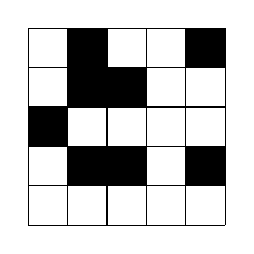
\begin{tikzpicture}[scale=0.5]
\fill[black] (1,1) rectangle (2,2);
\fill[black] (1,4) rectangle (2,5);
\fill[black] (4,1) rectangle (5,2);
\fill[black] (4,4) rectangle (5,5);
\fill[black] (1,3) rectangle (2,4);
\fill[black] (2,3) rectangle (3,4);
\fill[black] (2,1) rectangle (3,2);
\fill[black] (0,2) rectangle (1,3);
\draw (0,0) grid (5,5);
\end{tikzpicture}
\end{center}
次のようなサブグリッドが存在します。
\begin{center}
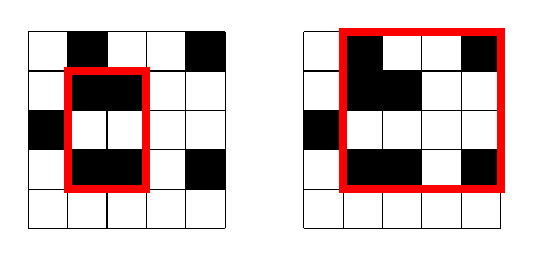
\begin{tikzpicture}[scale=0.5]
\fill[black] (1,1) rectangle (2,2);
\fill[black] (1,4) rectangle (2,5);
\fill[black] (4,1) rectangle (5,2);
\fill[black] (4,4) rectangle (5,5);
\fill[black] (1,3) rectangle (2,4);
\fill[black] (2,3) rectangle (3,4);
\fill[black] (2,1) rectangle (3,2);
\fill[black] (0,2) rectangle (1,3);
\draw (0,0) grid (5,5);

\fill[black] (7+1,1) rectangle (7+2,2);
\fill[black] (7+1,4) rectangle (7+2,5);
\fill[black] (7+4,1) rectangle (7+5,2);
\fill[black] (7+4,4) rectangle (7+5,5);
\fill[black] (7+1,3) rectangle (7+2,4);
\fill[black] (7+2,3) rectangle (7+3,4);
\fill[black] (7+2,1) rectangle (7+3,2);
\fill[black] (7+0,2) rectangle (7+1,3);
\draw (7+0,0) grid (7+5,5);

\draw[color=red,line width=1mm] (1,1) rectangle (3,4);
\draw[color=red,line width=1mm] (7+1,1) rectangle (7+5,5);
\end{tikzpicture}
\end{center}

この問題を解く$O(n^3)$時間のアルゴリズムは簡単です。
行のすべての$O(n^2)$組を調べ、各組$(a, b)$について、
両方の行で黒マスを含む列の数を$O(n)$時間で算出します。
以下のコードでは、$\texttt{color}[y][x]$が $y$ 行 $x$ 列の色を表すと仮定しています。
\begin{lstlisting}
int count = 0;
for (int i = 0; i < n; i++) {
    if (color[a][i] == 1 && color[b][i] == 1) count++;
}
\end{lstlisting}
そして、$\texttt{count}(\texttt{count}-1)/2$個の黒い角を持つサブグリッドが答えです。
サブグリッドを形成するために、そのうちの任意の2個を選んでいるためです。

このアルゴリズムを最適化するために、
グリッドを列のブロックに分割し、
各ブロックが連続する$N$個の列で構成されるようにしましょう。
そして、各列は、正方形の色を表す$N$ビット数のリストとして格納します。
これで、$N$個の列をビット演算で同時に処理できるようになりました。
以下のコードでは、$\texttt{color}[y][k]$が$N$個の色のブロックをビットで表しています。

\begin{lstlisting}
int count = 0;
for (int i = 0; i <= n/N; i++) {
    count += __builtin_popcount(color[a][i]&color[b][i]);
}
\end{lstlisting}
これは$O(n^3/N)$で動作します。

サイズ$2500 \times 2500$のランダムなグリッドを生成し、
オリジナルとビット最適化された実装を比較しました。
オリジナルのコードが$29.6$秒かかったのに対し、
ビット最適化版は$N = 32$ (int 数)で$3.1$秒、$N = 64$ (long 長数)で$1.7$ 秒で済みました。

\section{動的計画法へのビット演算の利用 - Dynamic programming}

ビット演算は動的計画法においても要素の部分集合を含む状態を整数で保存できるため、
効率的で便利な実装出来ることがあります。
ビット演算と動的計画法の組み合わせの例について見ていきましょう。

\subsubsection{最適な選択 - Optimal selection}

最初の例として、次の問題を考えます。
$n$日間にわたる$k$個の商品の価格が与えられており、
各商品をちょうど1回買いたい。
しかし1日に買うことができるのは1個までである。最小の合計金額は?
例えば,次のようなシナリオを考えることにします。($k = 3$, $n = 8$).

\begin{center}
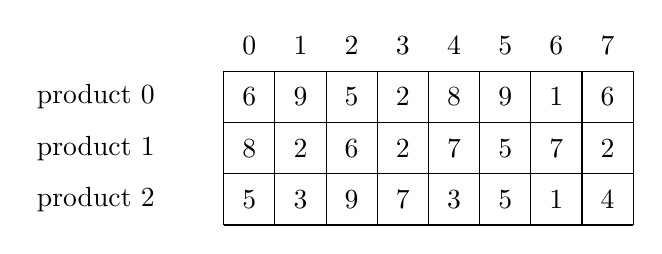
\begin{tikzpicture}[scale=.65]
    \draw (0, 0) grid (8,3);
    \node at (-2.5,2.5) {product 0};
    \node at (-2.5,1.5) {product 1};
    \node at (-2.5,0.5) {product 2};

    \foreach \x in {0,...,7}
        {\node at (\x+0.5,3.5) {\x};}
    \foreach \x/\v in {0/6,1/9,2/5,3/2,4/8,5/9,6/1,7/6}
        {\node at (\x+0.5,2.5) {\v};}
    \foreach \x/\v in {0/8,1/2,2/6,3/2,4/7,5/5,6/7,7/2}
        {\node at (\x+0.5,1.5) {\v};}
    \foreach \x/\v in {0/5,1/3,2/9,3/7,4/3,5/5,6/1,7/4}
        {\node at (\x+0.5,0.5) {\v};}
\end{tikzpicture}
\end{center}
このシナリオでは$5$が答えです。
\begin{center}
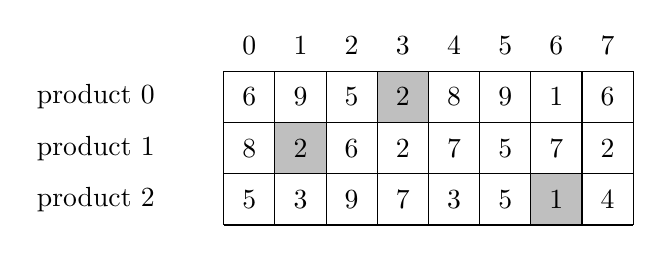
\begin{tikzpicture}[scale=.65]
    \fill [color=lightgray] (1, 1) rectangle (2, 2);
    \fill [color=lightgray] (3, 2) rectangle (4, 3);
    \fill [color=lightgray] (6, 0) rectangle (7, 1);
    \draw (0, 0) grid (8,3);
    \node at (-2.5,2.5) {product 0};
    \node at (-2.5,1.5) {product 1};
    \node at (-2.5,0.5) {product 2};

    \foreach \x in {0,...,7}
        {\node at (\x+0.5,3.5) {\x};}
    \foreach \x/\v in {0/6,1/9,2/5,3/2,4/8,5/9,6/1,7/6}
        {\node at (\x+0.5,2.5) {\v};}
    \foreach \x/\v in {0/8,1/2,2/6,3/2,4/7,5/5,6/7,7/2}
        {\node at (\x+0.5,1.5) {\v};}
    \foreach \x/\v in {0/5,1/3,2/9,3/7,4/3,5/5,6/1,7/4}
        {\node at (\x+0.5,0.5) {\v};}
\end{tikzpicture}
\end{center}

例えば,上のシナリオでは price[2][3] = 7です。
この関数を用いると,問題の解は total({0 ... k - 1}, n - 1) となります。
空集合を買うにはコストがかからないのでtotal((/), d) = 0、
初日に商品を1つ買う方法は1つなのでtotal({x}, 0) = price[x][0] として良いです。
そうすると、次のような漸化式をが利用できます。

ここでは$\texttt{price}[x][d]$は$d$での$x$の価格を示すとしましょう。
例えば,上のシナリオでは$\texttt{price}[2][3] = 7$です。
$\texttt{total}(S,d)$を、$d$日目時点での部分集合$S$を買うための最小のコストとしましょう。
これを用いると$\texttt{total}(\{0 \ldots k-1\},n-1)$が求めたい値となります。

まず、空集合を買うにはコストがかからないので$\texttt{total}(\emptyset,d) = 0$として良いです。
初日に商品を1つ買う方法は1つなので$\texttt{total}(\{x\},0) = \texttt{price}[x][0]$です。
そうすると、次のような漸化式となります。
\begin{equation*}
\begin{split}
\texttt{total}(S,d) = \min( & \texttt{total}(S,d-1), \\
& \min_{x \in S} (\texttt{total}(S \setminus x,d-1)+\texttt{price}[x][d]))
\end{split}
\end{equation*}
これは、$d$日にどの商品も買わないか、$S$に属する商品$x$を買うかのどちらかを意味します。
後者の場合、$x$を$S$から外し、$x$の価格を合計価格に加算します。

では動的計画法で関数の値を計算するための配列を用意しましょう。
\begin{lstlisting}
int total[1<<K][N];
\end{lstlisting}
ここで、$K$と$N$は適当な大きさの定数です。
配列の最初の次元は,部分集合のビット表現に対応します。

まず、$d=0$の場合は、以下のように処理することができます。
\begin{lstlisting}
for (int x = 0; x < k; x++) {
    total[1<<x][0] = price[x][0];
}
\end{lstlisting}
そして次のように書くことが出来ます。
\begin{lstlisting}
for (int d = 1; d < n; d++) {
    for (int s = 0; s < (1<<k); s++) {
        total[s][d] = total[s][d-1];
        for (int x = 0; x < k; x++) {
            if (s&(1<<x)) {
                total[s][d] = min(total[s][d],
                                    total[s^(1<<x)][d-1]+price[x][d]);
            }
        }
    }
}
\end{lstlisting}
これは$O(n 2^k k)$で動作します。

\subsubsection{順列からの集合 - From permutations to subsets}

動的計画法を用いると、
順列の繰り返しを部分集合の繰り返しに変更することができる場合があります。\footnote{This technique was introduced in 1962
by M. Held and R. M. Karp \cite{hel62}.}
順列の組み合わせ数である$n!$はとても大きな数となり、部分集合の組み合わせ数である$2^n$ よりもずっと大きくなるので非常に有効な方法です。
たとえば、$n = 20$として$n! \approx 2.4 \cdot 10^{18}$ であり、 $2^n \approx 10^6$です。
したがって、ある種の$n$の値に対して、部分集合は効率的に調べられるが、順列を調べることは困難です。

最大重量$x$のエレベータがあり、
1階から最上階まで行きたい体重が既知の$n$人がいるとする問題を考えます。
人々が最適な順序でエレベーターに乗り込む場合、必要な最小の乗車回数は何回ですか?

例えば、$x=10$、$n=5$で、重みは以下の通りだとしましょう。
\begin{center}
\begin{tabular}{ll}
person & weight \\
\hline
0 & 2 \\
1 & 3 \\
2 & 3 \\
3 & 5 \\
4 & 6 \\
\end{tabular}
\end{center}
この場合、最小の解は2です。最適な順序の1つは
$\{0,2,3,1,4\}$で、これは人々を2分割し、最初に
$\{0,2,3\}$(合計重量10)、次に
$\{1,4\}$(合計重量9)で運べば良いです。

この問題は、$n$人の可能な順列をすべてテストすることにより、$O(n! n)$時間で簡単に解くことがでます。
しかし、動的計画法を使って、より効率的な$O(2^n n)$時間のアルゴリズムを得ることもできます。
そのアイデアは、人の各サブセットについて、必要な最小乗車数と最後のグループで乗車する人々の最小重量という2つの値を計算することです。

ここで、$\texttt{weight}[p]$を人物 $p$ の重みとしましょう。
また、部分集合 $S$ の最小乗車数を$\texttt{rides}(S)$ 、最後の乗車の重みを $\texttt{last}(S)$  とします。

例えば、上記のシナリオの場合は以下のようになります。
\[ \texttt{rides}(\{1,3,4\})=2 \hspace{10px} \textrm{かつ}
\hspace{10px} \texttt{last}(\{1,3,4\})=5,\]
なぜなら最適な乗り物は$\{1,4\}$ と $\{3\}$であり、
2番目の乗り物は重み5だからである。もちろん、我々の最終目標は$\texttt{rides}(\{0 \ldots n-1\})$の値を計算することです。

関数の値を再帰的に計算し、
動的計画法を適用すればよいです。
これは、$S$に属するすべての人を調べて、
最後にエレベーターに入る人$p$を最適に選ぶというアルゴリズムです。
そのような選択のたびに,より小さな人々の部分集合に対する部分問題が生じます。
$\texttt{last}(S \setminus p)+\texttt{weight}[p] \le x$ならば、$p$ を最後に乗る人に加えることができます。
そうでなければ、最初はpしか乗っていない新しいカゴを確保しないとなりません。動的計画法を実装するために、次のような配列を用意します。
\begin{lstlisting}
pair<int,int> best[1<<N];
\end{lstlisting}
各分割集合 $S$ に対して$(\texttt{rides}(S),\texttt{last}(S))$のペアを含みます。
空のグループに対する値を以下のように設定します。
\begin{lstlisting}
best[0] = {1,0};
\end{lstlisting}
そして次のように計算ができます。
\begin{lstlisting}
for (int s = 1; s < (1<<n); s++) {
    // initial value: n+1 rides are needed
    best[s] = {n+1,0};
    for (int p = 0; p < n; p++) {
        if (s&(1<<p)) {
            auto option = best[s^(1<<p)];
            if (option.second+weight[p] <= x) {
                // add p to an existing ride
                option.second += weight[p];
            } else {
                // reserve a new ride for p
                option.first++;
                option.second = weight[p];
            }
            best[s] = min(best[s], option);
        }
    }
}
\end{lstlisting}
このループは、$S_1$ and $S_2$のような任意の2つの部分集合$S_1$ と$S_2$
に対して、$S_2$ の前に$S_1$ を処理することを保証できます。
動的計画法は正しい順序で値を計算されます。

\subsubsection{サブセットのカウントCounting subsets}

最後の問題です。
$X=\{0 \ldots n-1\}$として$S \subset X$
ここで各サブセットには$\texttt{value}[S]$の価値割り当てられているとします。
私たちのタスクは全ての$S$に対して以下を計算することです。
\[\texttt{sum}(S) = \sum_{A \subset S} \texttt{value}[A],\]
つまり、$S$の部分集合の価値総和です。

例えば、$n=3$の時、以下のように値を割り当てます。
\begin{multicols}{2}
\begin{itemize}
\item $\texttt{value}[\emptyset] = 3$
\item $\texttt{value}[\{0\}] = 1$
\item $\texttt{value}[\{1\}] = 4$
\item $\texttt{value}[\{0,1\}] = 5$
\item $\texttt{value}[\{2\}] = 5$
\item $\texttt{value}[\{0,2\}] = 1$
\item $\texttt{value}[\{1,2\}] = 3$
\item $\texttt{value}[\{0,1,2\}] = 3$
\end{itemize}
\end{multicols}
このケースでは、以下のように計算できます。
\begin{equation*}
\begin{split}
\texttt{sum}(\{0,2\}) &= \texttt{value}[\emptyset]+\texttt{value}[\{0\}]+\texttt{value}[\{2\}]+\texttt{value}[\{0,2\}] \\ 
                      &= 3 + 1 + 5 + 1 = 10.
\end{split}
\end{equation*}

サブセットは全部$2^n$あるので、
1つの可能な解決策は、サブセットのすべてのペアを$O(2^{2n})$時間で処理することです。
動的計画法を用いると、$O(2^n n)$時間で解くことができます。
このアイデアは、$S$から削除される可能性のある要素が制限されているということです。

例えば,Sから要素0 ... kだけを取り除いてもよいという制限のあるSの部分集合の値の総和をpartial(S, k)とする.
ここで、$\texttt{partial}(S,k)$を、
集合Sから$0 \ldots k$取り除いて良いものとしましょう。
\[\texttt{partial}(\{0,2\},1)=\texttt{value}[\{2\}]+\texttt{value}[\{0,2\}],\]

というのは、要素$0 \ldots 1$だけを削除することができるからです
ここで、\texttt{sum}は\texttt{partial}を使って表現できます。
\[\texttt{sum}(S) = \texttt{partial}(S,n-1).\]
初期値は
\[\texttt{partial}(S,-1)=\texttt{value}[S],\]
とします。この場合、$S$から要素を削除することはできないからです。
一般的な場合、以下の再帰で表現できます。
\begin{equation*}
    \texttt{partial}(S,k) = \begin{cases}
               \texttt{partial}(S,k-1) & k \notin S \\
               \texttt{partial}(S,k-1) + \texttt{partial}(S \setminus \{k\},k-1) & k \in S
           \end{cases}
\end{equation*}
ここで $k$に注目します。
 $k \in S$の場合、$S$から$k$消すか残すかを選択することが出来ます。

ここで和の計算を実装するのに特に賢い方法があります。
\begin{lstlisting}
int sum[1<<N];
\end{lstlisting}
各サブセットの合計を含むことになります。配列は以下のように初期化されます。
\begin{lstlisting}
for (int s = 0; s < (1<<n); s++) {
    sum[s] = value[s];
}
\end{lstlisting}
次のように処理を行います。
\begin{lstlisting}
for (int k = 0; k < n; k++) {
    for (int s = 0; s < (1<<n); s++) {
        if (s&(1<<k)) sum[s] += sum[s^(1<<k)];
    }
}
\end{lstlisting}
このコードは、$k=0 \ldots n-1$の
$\texttt{partial}(S,k)$の値を配列の和に計算します。
$\texttt{partial}(S,k)$は常に$\texttt{partial}(S,k-1)$に基づいているので、配列\texttt{sum}を再利用でき、非常に効率的に動作します。
